\subsection*{Teil B: Zylinderberechnungen - Grundlagen (30 Minuten)}

\begin{enumerate}[label=\arabic*., resume]

    \item \textbf{Ergänze die Formelsammlung für den Zylinder:}
    \vspace{0.5cm}

    \begin{center}
        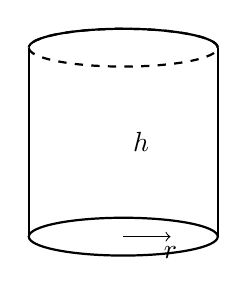
\begin{tikzpicture}[scale=0.8]
            \draw[thick] (0,0) ellipse (1.5 and 0.3);
            \draw[thick] (-1.5,0) -- (-1.5,3);
            \draw[thick] (1.5,0) -- (1.5,3);
            \draw[thick,dashed] (0,3) ellipse (1.5 and 0.3);
            \draw[thick] (-1.5,3) arc (180:0:1.5 and 0.3);
            \draw (0,1.5) node[right] {$h$};
            \draw (0.75,0) node[below] {$r$};
            \draw[->] (0,0) -- (0.75,0);
        \end{tikzpicture}
    \end{center}

    \begin{tabular}{ll}
        Grundfläche: & $G = \pi r^2$ \\[1ex]
        Mantelfläche: & $M = 2\pi r \cdot h$ \\[1ex]
        Oberfläche: & $O = 2G + M = 2\pi r^2 + 2\pi rh = 2\pi r($ \underline{\hspace{2cm}} $)$ \\[1ex]
        Volumen: & $V = G \cdot h =$ \underline{\hspace{3cm}}
    \end{tabular}

    \vspace{1cm}

    \item \textbf{Berechne für die gegebenen Zylinder:}
    \vspace{0.5cm}

    \begin{enumerate}[label=\alph*)]
        \item $r = 4$ cm, $h = 10$ cm

        Grundfläche: $G = \pi \cdot 4^2 = 16\pi \approx$ \underline{\hspace{2cm}} cm$^2$

        Mantelfläche: $M = 2\pi \cdot 4 \cdot 10 = 80\pi \approx$ \underline{\hspace{2cm}} cm$^2$

        Oberfläche: $O = 2 \cdot 16\pi + 80\pi = 112\pi \approx$ \underline{\hspace{2cm}} cm$^2$

        Volumen: $V = 16\pi \cdot 10 = 160\pi \approx$ \underline{\hspace{2cm}} cm$^3$

        \vspace{0.8cm}
        \item $d = 12$ cm, $h = 8$ cm (also $r = 6$ cm)

        Grundfläche: $G =$ \underline{\hspace{2cm}} cm$^2$

        Mantelfläche: $M =$ \underline{\hspace{2cm}} cm$^2$

        Oberfläche: $O =$ \underline{\hspace{2cm}} cm$^2$

        Volumen: $V =$ \underline{\hspace{2cm}} cm$^3$
    \end{enumerate}

    \vspace{1cm}

    \item \textbf{Zeichne das Netz eines Zylinders:}
    \vspace{0.5cm}

    Zylinder: $r = 2$ cm, $h = 5$ cm

    Umfang der Grundfläche: $U = 2\pi \cdot 2 = 4\pi \approx 12{,}57$ cm

    \vspace{0.5cm}

    \begin{center}
        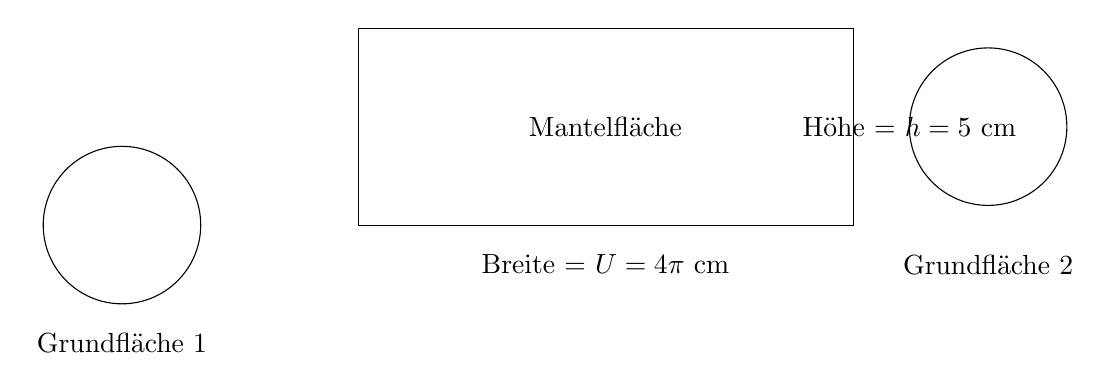
\begin{tikzpicture}[scale=0.5]
            % Grundkreis 1
            \draw (0,0) circle (2);
            \node at (0,-3) {Grundfläche 1};

            % Mantelrechteck
            \draw (6,0) rectangle (18.57,5);
            \node at (12.28,2.5) {Mantelfläche};
            \node at (12.28,-1) {Breite = $U = 4\pi$ cm};
            \node at (20,2.5) {Höhe = $h = 5$ cm};

            % Grundkreis 2  
            \draw (22,2.5) circle (2);
            \node at (22,-1) {Grundfläche 2};
        \end{tikzpicture}
    \end{center}

\end{enumerate}